\section{Data collection}
\label{sec:data-collecting}
In order to build a system to transcribe beatboxing by amateurs we had to gather a dataset based on this aspect. 
Non-probability sampling was used to collect the data, in which 19 people participated, and it took place in the main building of Aalborg University Copenhagen. 

The participants were placed in a chair surrounded by small partition walls (see cfigure \ref{data-collection-pic}) to limit noise from the surroundings. They were asked to produce 5-10 of each of the three sounds, and also to perform a self-improvised short mix of the sounds.

To record the beatboxing sequences we used a e815-S dynamic cardioid microphone attached to an H4n portable recorder. The sampling rate was 96 kHz and 24 bit precision.

The gathered data was collected on one track used as a database for our system. In order to utilize this database the sound file had to be manually annotated. This means that for each sound its onset was denoted and saved, and the type of sound labelled according to the three sound classes. This was done using Sonic Visualiser\footnote{\url{http://www.sonicvisualiser.org/}}, which generated a text file with the needed information.

\begin{figure}[h]
	\begin{center}
		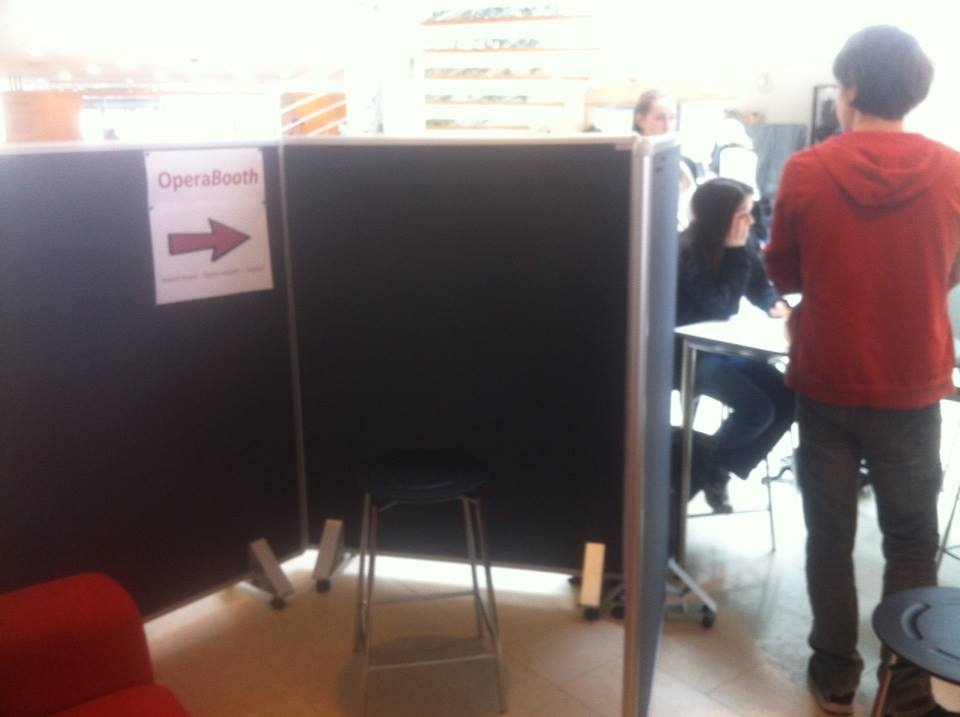
\includegraphics[height=5cm]{fig/dataset_collection.JPG}
		\caption{Data collection booth.}
		\label{data-collection-pic}
	\end{center}
\end{figure}